\documentclass[11pt]{ctexbeamer}
\usetheme{Darmstadt}
\usepackage{amsmath}
\usepackage{amsfonts}
\usepackage{amssymb}
\usepackage{graphics}
\usepackage{color}
\usepackage{amsmath,amsthm,amsfonts,amssymb,bm}
% \usepackage{newtxtext,newtxmath}
\usepackage{mathptmx}
\usepackage{mathptmx}

\addtobeamertemplate{block begin}{%
  \setlength{\textwidth}{0.9\textwidth}%
}{}

\addtobeamertemplate{block alerted begin}{%
  \setlength{\textwidth}{0.9\textwidth}%
}{}

\addtobeamertemplate{block example begin}{%
  \setlength{\textwidth}{0.9\textwidth}%
}{}
\author{周亮}
\title{近期工作总结}
\graphicspath{{fig/}}
\setbeamercovered{transparent}
\setbeamertemplate{navigation symbols}{}
\logo{
\includegraphics[scale=0.1]{icons_nudt.jpg}}
\institute{102教研室}
\date{\today}
\setmainfont{Times New Roman}
\setsansfont{Arial}
\setmonofont{Courier New}
%%%% Using Office Family Fonts
\setCJKmainfont[BoldFont={STZhongsong}]{SimSun}
\setCJKsansfont{SimHei} % Hei
\setCJKmonofont{FangSong} % Fangsong
%%%% alias
\setCJKfamilyfont{song}{SimSun}
\setCJKfamilyfont{hei}{SimHei}
\setCJKfamilyfont{fs}{FangSong} % fang-song
\setCJKfamilyfont{kai}{KaiTi} % Kai

\begin{document}
\begin{frame}
	\titlepage
\end{frame}

\begin{frame}
	\tableofcontents
\end{frame}

\section{月地转移轨道初步设计}
\begin{frame}{双二体假设下的计算模型}
	\begin{itemize}
		\item 优化变量选择\par
		      出口点时间$ t_B $,出口点在白道系下的升交点角距$ u $,白道系下的速度$ v_{si} $
		\item 优化目标\par
		      $ J=\Delta v $加速点速度增量
		\item 约束条件\par
		      不等式约束:\\总飞行时间$ T_{\max} $,燃料限制$\Delta v_{\max}  $,航程角约束$ \delta R_{\min}\to  \delta R_{\max}$\\
		      等式约束:\\近地距,与再入角相关$ r_p=r_e\cos \gamma^2 $
	\end{itemize}
\end{frame}

\begin{frame}{返回轨道设计程序结构}
	\begin{block}{模块划分}
		\begin{enumerate}
			\item 初始化部分:Earth,Mission等参数存于结构体
			\item 优化量的范围:lb,ub
			\item 优化算法:ga,sqp等
			\item 目标函数和各种非线性约束:ObjFun,ConFun
			\item 描述求解模型的Dynamic函数
		\end{enumerate}
	\end{block}
\end{frame}

\begin{frame}{一些关键的函数}
	\begin{block}{Dynamic函数中}
		\begin{itemize}
			\item 星历的调用:pleph.m,注意输出的单位km
			\item 时间系统的转换:UTC、TDB等
			\item 月心段轨道参数:双曲轨道计算公式
			\item 地心段轨道参数:椭圆轨道计算公式、或双曲轨道计算公式
			原因:解决优化问题,提供的初值一般不能满足椭圆轨道返回
			\item 着陆场和再入点参数:解决航程约束问题
		\end{itemize}
	\end{block}
\end{frame}

\begin{frame}{Debug中遇到问题}
	\begin{block}{常见易犯的错误}
		\begin{itemize}
			\item 利用反三角函数求解的角度范围\\
			$ \arctan,\arcsin,\arccos $等等
			\item 角度范围的限定\\
			通常角度$[0~2\pi],[-\pi,\pi]$几种标准,在涉及到角度的加减运算时需要注意,在本文的程序中轨道根数相关的角度信息均设置在$[0~2\pi]$,$ \Omega,\omega,f $
			\item 解决地心段轨道的问题\\
			可能存在椭圆和双曲线两种轨道,因此在计算地心段参数,需要同时考虑两种情况予以判断
		\end{itemize}
	\end{block}
\end{frame}
\begin{frame}{初步设计结果}
	\begin{block}{结果对比}
		仿真条件设置和沈论文保持一致

		
	\end{block}
	气动系数的插值,导致伪谱程序求解慢,效率差10倍左右\\
	能否采用拟合的方式\\
	
	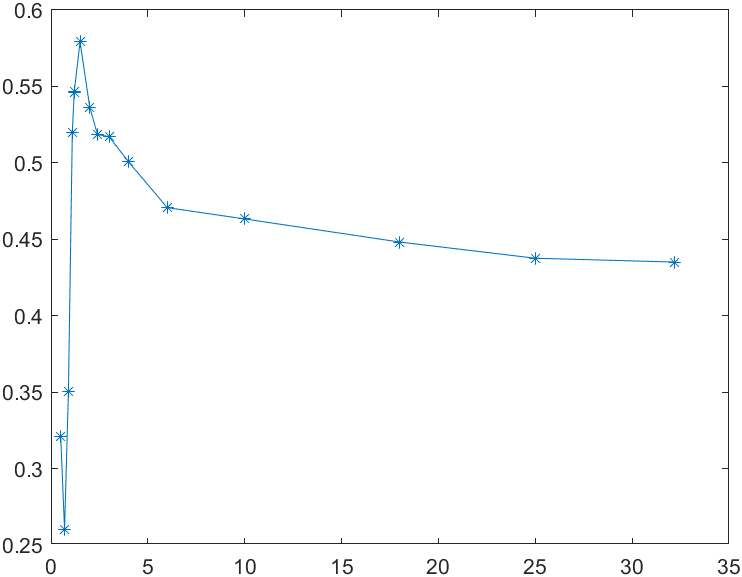
\includegraphics[height=.4\textheight]{Ma_Cl.png}
	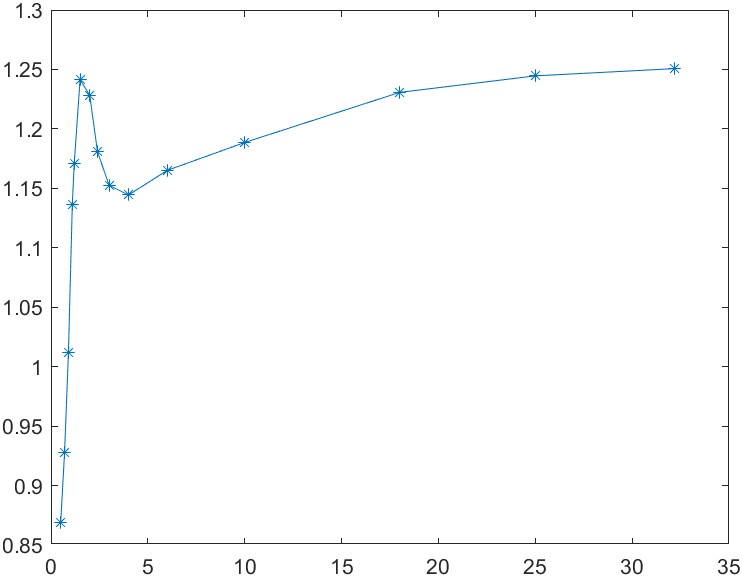
\includegraphics[height=.4\textheight]{Ma_Cd.png}

\end{frame}

\begin{frame}{工作计划}
	\begin{block}{}
		\begin{enumerate}
			\item 明确采用什么模型进行空间轨道设计与再入轨道设计,(双二体模型或者考虑摄动的精确模型)
			\item 确定再入瞄准点的选择方法(是否考虑其中的黄金再入走廊等方式)
			\item 完成再入可达域的绘图分析部分
		\end{enumerate}
	\end{block}
\end{frame}
\end{document}